\chapter{Simulation of Bit Error Patterns}

Considering the difficulty of replicating the exact link twice, we wrote a simple trace-based simulator that allows to apply the same bit error pattern from a real experiment onto new payload link-by-link.
This way we can keep the temporal variations of the link intact and single out the effect of bit error patterns on different payloads.

In this chapter we will describe how we model the patterns described in Section~\ref{sec:bit_error_patterns} to simulate them on new payload, and what the limitations of this method are.

\section{Design}

\subsection{Pattern extraction}

For every original link in the experiment log, we count the bit errors per bit per symbol.
This results in a table of 16 symbols, each of which has 4 entries, one for every bit in the symbol.
The table is then normalized for the occurance of the respective symbol to yield a relative bit error occurance per symbol for this specific link.

This table can be averaged over several links using a sliding window, which reduces noise and increases probability of seeing all symbols with their respective bit error patterns.
Note, that this creates a table of \emph{average} bit error probabilities per symbol over one or several links.
Therefore we also collect the distribution of bit error burst length over this window.

\subsection{Pattern application}

Every logged link, consisting out of transmitted and received messages, is copied and its transmitted payload replaced by a new payload.
Then a corruption pattern is generated by randomly corrupting each new symbol with the probability defined in the bit error table.
This corruption pattern consists mostly out of single bit errors, therefore for every single bit error, we randomly stretch it in length proportionately to the burst error distribution of the original link.
The corruption sequence is applied to the transmitted payload and written to the received message of the copied link.
Since the original link is copied, its metadata, such as link qualifiers, temperature, transmission power, is retained.

\subsection{Limitations}

We map bit error distribution per symbol, therefore every symbol must be available in the original payload for this table to be complete.
Experiment logs with constant payload in which not every symbol is available should be avoided.
For random payload our payload size of 93 bytes yields 186 symbols, for which it is unlikely to not see every 16 symbols at least once.

Another limitation is our modelling of bit error burstiness.
Schmidt~\etal~\cite{Schmidt2013} showed in their research that burst errors are not independently distributed, but occur more often within the boundaries of a symbol (4 bits) and less often crossing this boundary.
By ``simply'' applying the collected bit error table by symbol onto new payload, we are effectively interleaving the original burst errors and therefore obscuring this property of the original link.
With our simple simulation, we can only add burst errors to correct for relative occurance compared to the original frame, but not willfully ``place'' these burst errors at the correct position to achieve the destinct burst error properties of the original link.


\section{Accuracy}

To evaluate the performance of the simulator, we used the experiment traces containing constant payloads as well as pseudo-random payloads.
By tuning the link input window size and the aggression of the burst error generator, we were able to replicate similar enough bit error patterns for our purposes.
We found best accuracy with a window size of two links and three passes of the burst generator.

Figure~\ref{fig:8mote_xl_xor_simulation} shows the bit error pattern resulting of simulating the experiment described in Section~\ref{sec:effects_of_board_layout}.
Compared to the original pattern in Figure~\ref{fig:8mote_bit_errors_xl}, the simulation generates a less noisy footprint with less amplitude, which makes the differences in symbols clearly visible.
This is, of course, due to the averaging during the symbol error construction which is accompanied with the smoothing of these values.

The limitations of our burst error modelling clearly show in the burst error graph of the simulated 

\begin{figure}[ht]
	\subfigure[Simulated bit error pattern.] {
    	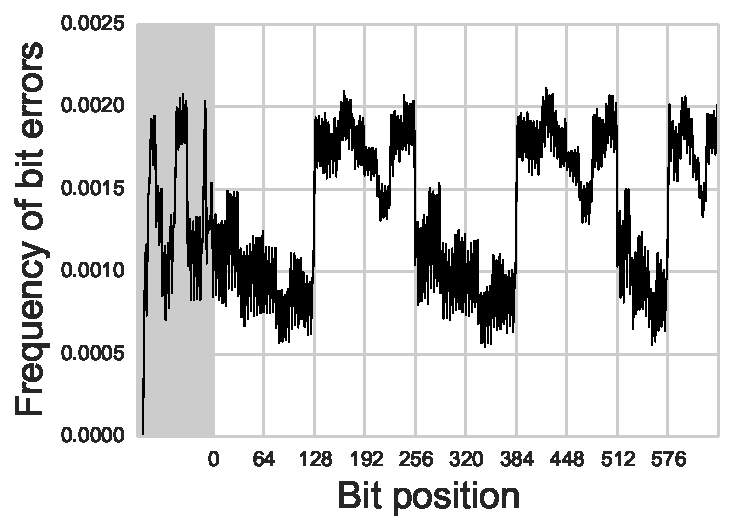
\includegraphics[width=0.5\columnwidth]{figures/8mote_0-5_xor_simulation}
    	\label{fig:8mote_xl_xor_simulation}
    }
    \subfigure[Simulated burst error distribution.] {
	    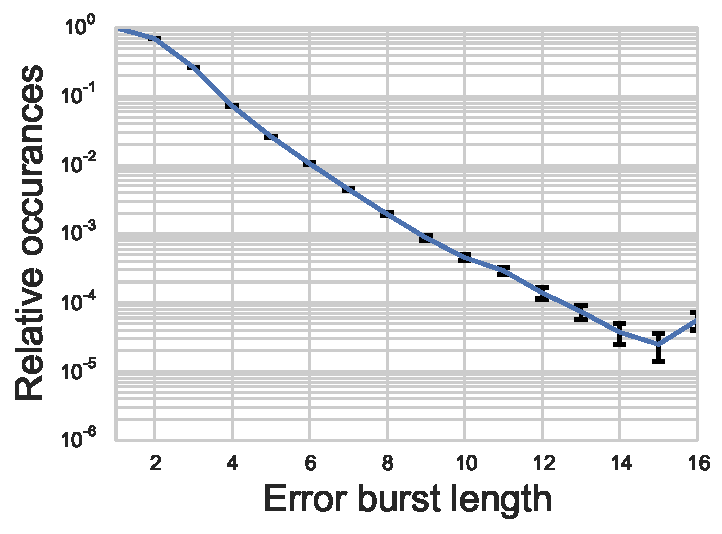
\includegraphics[width=0.5\columnwidth]{figures/8mote_0-5_burst_simulation}
	    \label{fig:8mote_xl_burst_simulation}
	}
	\caption{Bit error patterns of simulated constant payload using traces with constant payload.}
	\label{fig:8mote_bit_error_simulation}
\end{figure}

